%	-------------------------------------------------------------------------------
% 
%
%
%
%
%
%
%
%
%
%	-------------------------------------------------------------------------------

	\documentclass[12pt, a4paper, oneside]{book}
%	\documentclass[12pt, a4paper, landscape, oneside]{book}

		% --------------------------------- 페이지 스타일 지정
		\usepackage{geometry}
%		\geometry{landscape=true	}
		\geometry{top 		=10em}
		\geometry{bottom		=10em}
		\geometry{left		=8em}
		\geometry{right		=8em}
		\geometry{headheight	=4em} % 머리말 설치 높이
		\geometry{headsep		=2em} % 머리말의 본문과의 띠우기 크기
		\geometry{footskip		=4em} % 꼬리말의 본문과의 띠우기 크기
% 		\geometry{showframe}
	
%		paperwidth 	= left + width + right (1)
%		paperheight 	= top + height + bottom (2)
%		width 		= textwidth (+ marginparsep + marginparwidth) (3)
%		height 		= textheight (+ headheight + headsep + footskip) (4)



		%	===================================================================
		%	package
		%	===================================================================
%			\usepackage[hangul]{kotex}				% 한글 사용
			\usepackage{kotex}						% 한글 사용
			\usepackage[unicode]{hyperref}			% 한글 하이퍼링크 사용
			\usepackage{amssymb,amsfonts,amsmath}	% 수학 수식 사용

			\usepackage{scrextend}					% 
		
			\usepackage{enumerate}			%
			\usepackage{enumitem}			%
			\usepackage{tablists}			%	수학문제의 보기 등을 표현하는데 사용
										%	tabenum


		% ------------------------------ table 
			\usepackage{longtable}			%
			\usepackage{tabularx}			%

			\usepackage{setspace}			%
			\usepackage{booktabs}			% table
			\usepackage{color}				%
			\usepackage{multirow}			%
			\usepackage{boxedminipage}		% 미니 페이지
			\usepackage[pdftex]{graphicx}	% 그림 사용
			\usepackage[final]{pdfpages}	% pdf 사용
			\usepackage{framed}			% pdf 사용
			
			\usepackage{fix-cm}	
			\usepackage[english]{babel}
	
			\usepackage{tikz}%
			\usetikzlibrary{arrows,positioning,shapes}
			%\usetikzlibrary{positioning}
			

		% --------------------------------- 	page
			\usepackage{afterpage}			% 다음페이지가 나온면 어떻게 하라는 명령 정의 패키지
%			\usepackage{fullpage}			% 잘못 사용하면 다 흐트러짐 주의해서 사용
%			\usepackage{pdflscape}			% 
			\usepackage{lscape}			%	 


			\usepackage{blindtext}
	
		% --------------------------------- font 사용
			\usepackage{pifont}				%
			\usepackage{textcomp}
			\usepackage{gensymb}
			\usepackage{marvosym}






		% --------------------------------- 페이지 스타일 지정

		\usepackage[Sonny]		{fncychap}

			\makeatletter
			\ChNameVar	{\Large\bf}
			\ChNumVar		{\Huge\bf}
			\ChTitleVar	{\Large\bf}
			\ChRuleWidth	{0.5pt}
			\makeatother

%		\usepackage[Lenny]		{fncychap}
%		\usepackage[Glenn]		{fncychap}
%		\usepackage[Conny]		{fncychap}
%		\usepackage[Rejne]		{fncychap}
%		\usepackage[Bjarne]	{fncychap}
%		\usepackage[Bjornstrup]{fncychap}

		\usepackage{fancyhdr}
		\pagestyle{fancy}
		\fancyhead{} % clear all fields
		\fancyhead[LO]{\footnotesize \leftmark}
		\fancyhead[RE]{\footnotesize \leftmark}
		\fancyfoot{} % clear all fields
		\fancyfoot[LE,RO]{\large \thepage}
		%\fancyfoot[CO,CE]{\empty}
		\renewcommand{\headrulewidth}{1.0pt}
		\renewcommand{\footrulewidth}{0.4pt}
	
	
	
		% --------------------------------- 	section 스타일 지정
	
		\usepackage{titlesec}
		
		\titleformat*{\section}			{\large\bfseries}
		\titleformat*{\subsection}			{\normalsize\bfseries}
		\titleformat*{\subsubsection}		{\normalsize\bfseries}
		\titleformat*{\paragraph}			{\normalsize\bfseries}
		\titleformat*{\subparagraph}		{\normalsize\bfseries}
	
		\renewcommand{\thesection}			{\arabic{section}.}
		\renewcommand{\thesubsection}		{\thesection\arabic{subsection}.}
		\renewcommand{\thesubsubsection}	{\thesubsection\arabic{subsubsection}}
		
		\titlespacing*{\section} 			{0pt}{1.0em}{1.0em}
		\titlespacing*{\subsection}	  		{0ex}{1.0em}{1.0em}
		\titlespacing*{\subsubsection}		{0ex}{1.0em}{1.0em}
		\titlespacing*{\paragraph}			{0ex}{1.0em}{1.0em}
		\titlespacing*{\subparagraph}		{0ex}{1.0em}{1.0em}
	
	%	\titlespacing*{\section} 			{0pt}{0.0\baselineskip}{0.0\baselineskip}
	%	\titlespacing*{\subsection}	  		{0ex}{0.0\baselineskip}{0.0\baselineskip}
	%	\titlespacing*{\subsubsection}		{6ex}{0.0\baselineskip}{0.0\baselineskip}
	%	\titlespacing*{\paragraph}			{6pt}{0.0\baselineskip}{0.0\baselineskip}
	

		% --------------------------------- recommend		섹션별 페이지 상단 여백
		\newcommand{\SectionMargin}			{\newpage  \null \vskip 2cm}
		\newcommand{\SubSectionMargin}		{\newpage  \null \vskip 2cm}
		\newcommand{\SubSubSectionMargin}	{\newpage  \null \vskip 2cm}


	
		% --------------------------------- 장의 목차
		\usepackage{minitoc}
		\setcounter{minitocdepth}{1}    	% Show until subsubsections in minitoc
		\setlength{\mtcindent}{12pt} 		% default 24pt
	
	
		% --------------------------------- 	문서 기본 사항 설정
		\setcounter{secnumdepth}{3} 		% 문단 번호 깊이
		\setcounter{tocdepth}{3} 			% 문단 번호 깊이
		\setlength{\parindent}{0cm} 		% 문서 들여 쓰기를 하지 않는다.
		
		
		% --------------------------------- 	줄간격 설정
		\doublespace
%		\onehalfspace
%		\singlespace
		
		
% 	============================================================================== List global setting
%		\setlist{itemsep=1.0em}
	
% 	============================================================================== enumi setting

%		\renewcommand{\labelenumi}{\arabic{enumi}.} 
%		\renewcommand{\labelenumii}{\arabic{enumi}.\arabic{enumii}}
%		\renewcommand{\labelenumii}{(\arabic{enumii})}
%		\renewcommand{\labelenumiii}{\arabic{enumiii})}


	%	-------------------------------------------------------------------------------
	%		Vertical and Horizontal spacing
	%	-------------------------------------------------------------------------------
		\setlist[enumerate,1]	{ leftmargin=8.0em, rightmargin=0.0em, labelwidth=0.0em, labelsep=0.0em }
		\setlist[enumerate,2]	{ leftmargin=8.0em, rightmargin=0.0em, labelwidth=0.0em, labelsep=0.0em }
		\setlist[enumerate,3]	{ leftmargin=8.0em, rightmargin=0.0em, labelwidth=0.0em, labelsep=0.0em }
		\setlist[enumerate]	{ 	itemsep=1.0em, 
								leftmargin=6.0ex, 
								rightmargin=0.0em, 
								labelwidth=0.0em, 
								labelsep=4.0ex 
							}


	%	-------------------------------------------------------------------------------
	%		Label
	%	-------------------------------------------------------------------------------
%		\setlist[enumerate,1]{ label=\arabic*., ref=\arabic* }
%		\setlist[enumerate,1]{ label=\emph{\arabic*.}, ref=\emph{\arabic*} }
%		\setlist[enumerate,1]{ label=\textbf{\arabic*.}, ref=\textbf{\arabic*} }   	% 1.
%		\setlist[enumerate,1]{ label=\textbf{\arabic*)}, ref=\textbf{\arabic*)} }		% 1)
		\setlist[enumerate,1]{ label=\textbf{(\arabic*)}, ref=\textbf{(\arabic*)} }	% (1)
		\setlist[enumerate,2]{ label=\textbf{\arabic*)}, ref=\textbf{\arabic*)} }		% 1)
		\setlist[enumerate,3]{ label=\textbf{\arabic*.}, ref=\textbf{\arabic*.} }		% 1.

%		\setlist[enumerate,2]{ label=\emph{\alph*}),ref=\theenumi.\emph{\alph*} }
%		\setlist[enumerate,3]{ label=\roman*), ref=\theenumii.\roman* }


% 	============================================================================== itemi setting


	%	-------------------------------------------------------------------------------
	%		Vertical and Horizontal spacing
	%	-------------------------------------------------------------------------------
		\setlist[itemize]{itemsep=0.0em}






		% --------------------------------- recommend  글자 색깔지정 명령
		\newcommand{\red}		{\color{red}}			% 글자 색깔 지정
		\newcommand{\blue}		{\color{blue}}		% 글자 색깔 지정
		\newcommand{\black}	{\color{black}}		% 글자 색깔 지정
		\newcommand{\superscript}[1]{${}^{#1}$}

	
	
		% --------------------------------- 환경 정의 : 박스 치고 안의 글자 빨간색

			\newenvironment{BoxRedText}
			{ 	\setlength{\fboxsep}{12pt}
				\begin{boxedminipage}[c]{1.0\linewidth}
				\color{red}
			}
			{ 	\end{boxedminipage} 
				\color{black}
			}
			
			

% ------------------------------------------------------------------------------
% Begin document (Content goes below)
% ------------------------------------------------------------------------------
	\begin{document}
	
			\dominitoc
			

			\title{지각변형}
			\author{김대희}
			\date{2015년 8월}
			\maketitle


			\tableofcontents
			\listoffigures
			\listoftables

			

% ================================================= chapter 	====================
	\newpage
	\chapter{지각 변형}


	% -------------------------------------- page -------------------
	%	\nomtcrule         		% removes rules = horizontal lines
	%	\nomtcpagenumbers  % remove page numbers from minitocs
		\newpage
		\minitoc				% Creating an actual minitoc
	%	\doublespace


	% ------------------------------------------ section ------------ 
	\newpage  \null
	\section{관 입}




이미 생성된 암석 속으로 새로운 【 액체 】 또는 【 반액체 】 상태의 【 마그마 】가 뚫고 들어와 자리 잡으면 이를 【 관입 】이라 하며, 새로 자리한 암석을 【 관입암 】이라고 한다.


드물게 퇴적암이 만들어지는 과정에서도 위층은 굳었는데 아래층이 아직 굳지 않았을 때에, 지각변동으로 위층에 틈이 생기면 덜 굳은 아래층 암석의 일부가 그 틈 사이를 따라 위층으로 이동하여 자리 잡기도 한다. 이런 경우도 관입이라고 한다.




	% ------------------------------------------ section ------------ 
	\newpage  \null
	\section{엽 리}




	\subsection{엽리葉理}
葉 잎 엽  理 다스릴 리
널빤지 모양의 광물이 나란하게 배열되어 나타나는 구조. 
주로 변성암에 잘 나타난다.


	\subsection{엽리(foliation)}

① 변성암의 평행구조. 암석이 광역변성작용(廣域變成作用 ; 재결정작용)을 받아 온도와 압력이 변화하면  운모 같은 판상의 광물이 평행하게 배열되는 구조이다. 엽상구조라고도 한다.

엽리에 있어서 구성광물들이 세립이고 균질하게 배열된 평행구조를 【 편리 】(片理)라 하고, 유색광물과 무색광물이 서로 교대로 거친 줄무늬를 보여주는 것을 【 편마 】(片麻)구조라 한다.

② 빙하와 빙하가 서로 부딪혀 빙하 기저부에 생겨난 층리(層理) 모양의 구조. 이것은 빙하의 성장 때 생겨나는 층상구조와는 구별된다.




구성물질의 입도(粒度)나 조성의 차이 때문에 지층 중에 생긴 세밀한 줄무늬의 배열 상태를 말한다. 층리(層理) 중에서 최소단위의 것이다. 원래의 퇴적상태를 나타낸다. 이암(泥岩) 셰일이나 세립 사암 내에서 흔히 발견된다. 보통은 평행한 줄무늬를 이루나, 때로는 사교(斜交) 또는 수렴한다. 엽층이 생기는 원인은 여러 가지 물질의 공급(또는 퇴적) 속도의 변화에 있으며, 이와 같은 변화는 수류(水流)의 변화, 기후의 변화 등에 기인한다. 또한 빙하와 빙하가 서로 부딪쳐 빙하 기저부에 생겨난 층리모양의 구조이다. 이것은 빙하의 성장 때 생겨나는 층리구조와는 구별 된다
[네이버 지식백과] 엽리 [葉理, foliation] (자연지리학사전, 2006.5.25, 한울아카데미)


		\begin{figure}[h!]
		\caption{셰일 ( Shale ) 엽리가 잘 발달된 P일과 엽리면 위에 보존된 식물잎 화석}
		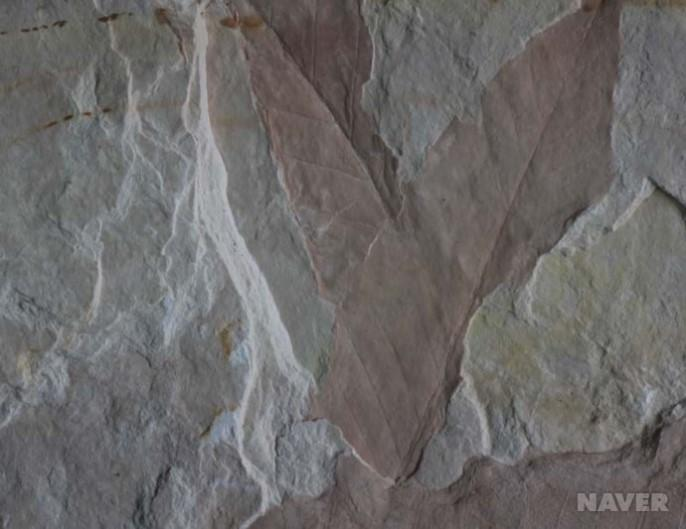
\includegraphics[width=1.0\textwidth]{./fig/fig-001.jpg}
		\end{figure}



	\subsection{엽리 [ 葉理, foliation ] }


구성물질의 입도(粒度)나 조성의 차이 때문에 지층 중에 생긴 세밀한 줄무늬의 배열 상태를 말한다. 층리(層理) 중에서 최소단위의 것이다. 

원래의 퇴적상태를 나타낸다. 

이암(泥岩) 셰일이나 세립 사암 내에서 흔히 발견된다. 보통은 평행한 줄무늬를 이루나, 때로는 사교(斜交) 또는 수렴한다. 엽층이 생기는 원인은 여러 가지 물질의 공급(또는 퇴적) 속도의 변화에 있으며, 이와 같은 변화는 수류(水流)의 변화, 기후의 변화 등에 기인한다. 또한 빙하와 빙하가 서로 부딪쳐 빙하 기저부에 생겨난 층리모양의 구조이다. 이것은 빙하의 성장 때 생겨나는 층리구조와는 구별된다.
(자연지리학사전, 2006.5.25, 한울아카데미)






	% ------------------------------------------ section ------------ 
	\newpage  \null
	\section{층리와 엽리의 구별}




1. 		층리와 엽리의 구별

암석이나 지층을 관찰하다 보면 층리나 엽리와 같은 평행한 줄무늬를 볼 수 있다. 두 줄무늬를 구별하는 방법을 알아보자. 

\paragraph{층리 : 퇴적물이 쌓이면서 만들어진 구조}
먼저 퇴적암에서 볼 수 있는 층리는 서로 다름 지층이 쌓여서 나타난다. 즉 퇴적암의 층리는 퇴적물이 쌓이면서 만들어진 구조이다.

\paragraph{엽리 : 압력을 받아 광물들이 수직방향으로 늘어서서 만들어진 줄늬}
그렇다면 변성암 ( 특히 편마암 )에 잘 나타나는 엽리는 어떻게 만들어질까? 엽리는 변성작용 중에 암석이 높은 압력을 받아서 광물들이 압력에 수직 방향으로 늘어서서 만들어진 줄무늬이다.




	% ------------------------------------------ section ------------ 
	\newpage  \null
	\section{층리}


1. 		층리

퇴적암의 특징으로는 차곡차곡 쌓인 구조가 나타난다는 것인데, 이것이 바로 【 층리 구조 】이다. 여기서 층이란 암질, 내부구조, 조직 등의 차이로 상하부가 구별되는 퇴적단위이다.

(1) 엽층리
층리의 두께가 1  이하이면 엽층리라 한다.







	% ------------------------------------------ section ------------ 
	\newpage  \null
	\section{엽 층 리( 葉層理, lamina )}




1. 		엽층리 [ 葉層理, lamina ] 

(1) 엽층리
층리의 두께가 1  이하이면 엽층리라 한다.

크기가 0.06 보다 작은 입자들로 구성된 퇴적암을 이질암이라고 하는데, 특히 얇은 엽츨 리가 발달하면서 이 면을 따라 판상의 쪼개짐이 있으면 셰일이라 부른다.



2. 엽층리 [ 葉層理, lamina ] 

퇴적물이나 퇴적암에서 식별할 수 있는 가장 얇은 퇴적 단위로서 색, 성분, 입자 크기에 의해 결정되는 두께 1 cm 이하의 층을 말한다. 

무기적 또는 유기적 기원에 의해서 탄산염암에서 엽층리가 생성된다. 유기적 기원의 엽층리는 조상대, 조간대 및 조하대에서 섬유상(filamentous)의 남조류(blue green algae)에 의해 생성된다. 섬유상의 남조류는 점액질로서 파도나 조석에 의해 운반되는 석회니를 결속시켜 유기물과 석회니로 구성된 엽리를 형성한다. 이러한 유기물과 석회니가 교호하면서 엽리가 발달하여 스트로마톨라이트(stromatolite)를 형성한다. 스트로마톨라이트는 그 형태에 따라 횡적 연결 반구형(laterally linked hemispheroid; LLH), 위로 쌓아진 반구형(stacked hemispheroid; SH) 그리고 구형(spheroidal structure; SS)으로 구분되는데 LLH는 조상대와 조간대, SH는 물의 순환이 좋지 않거나 증발이 많은 조간대 그리고 SS는 물의 요동이 많은 조하대에서 생성된다. 탄산염 엽층리와 관련되어 흔히 조안 구조(bird's-eye structure)가 분포하게 된다.
[네이버 지식백과] 엽층리 [葉層理, lamina] (지구과학사전, 2009.8.30, 북스힐)





	% ------------------------------------------ section ------------ 
	\newpage  \null
	\section{습곡}





지층이 수평 방향으로 양쪽에서 미는 힘을 오랫동안 강하게 받으면 지층은 휘어진다. 이렇게 구부러진 지층의 구조를 【 습곡 】이라고 한다.

습곡에서 위로 볼록한 부분을 【 배사 】, 아래로 볼록한 부분을 【 향사 】라고 한다. 그리고 배사와 향사 사이의 기울어진 부분을 【 날개 】라고 한다.





	% ------------------------------------------ section ------------ 
	\newpage  \null
	\section{단열 fracture}
	단열이란 암석이나 깨어져 생긴 면을 총칭하는 것으로 암반내에 발달하는 모든 깨어진 면들을 단열이라 할 수 있다.



	% ------------------------------------------ section ------------ 
	\newpage  \null
	\section{절리}


	암석의 갈라진 틈으로 양쪽 암체의 상대적 변위가 없는 것

	절리는 암석의 갈라진 틈으로서 절리면을 중심으로 양쪽 암체의 상대적 변위가 없는 것을 말한다.

	절리는 대개 모든 암석에서 발달하고 있으며
지하수의 흐름의 통로
풍화 진행의 방향성을 제공하며
서로 다른 방향의 절리에 의해 분리된 암괴를 형성한다.

절리는 지각 천부에서 발생하는 취성변형의 산물이며, 이 취성변형의 과정에서 ``전단응력''에 의해 생성된 절리를 ``전단절리'' ``인장응력'에 의해 생성된 절리를 ``인장절리''라고 한다.



	\subsection{판상절리}
화강암내에서 발달하는 판상절리

	\subsection{주상절리}
현무암내에서 발달하는 주상절리













% ================================================= chapter 	====================
	\newpage
	\chapter{단층}





	% ------------------------------------------ section ------------ 
	\newpage  \null
	\section{단층 일반}



1. 		단층


지층이 강한 힘을 오랫동안 받으면 그 힘을 견디지 못하고 끊어진다. 이때 생긴 틈을 경계로 양쪽 지층 덩어리가 상대적으로 이동해 어긋난 구조를 【 단층 】이라고 한다.


단층에서 두 개의 지층 덩어리가 서로 어긋난 면을 【 단층면 】이라 하며, 경사진 단층면을 기준으로 위쪽에 있는 지층 덩어리를 【 상반 】, 아래쪽에 있는 지층 덩어리를 【 하반 】이라고 한다.



2. 		정단층





3. 		역단층


전단층과 대조적으로 암석이 양쪽에서 미는 힘에 의해 변형된다면, 경사진 단층면을 경계로 위 부분의 암석이 상대적으로 밀려올라 갈 수 있다. 이러한 단층을 역단층이라 한다.




4. 		정단층과 역단층의 구별

지각변동이 일어나 지층의 【 횡압력 】이나 【 장력 】의 힘을 받아서 지층이 갈라져 어긋나는 단층현상에는 【 정단층 】과 【 역단층 】이 있다. 이들은 어떻게 만들어지며 어떻게 구별하는지 알아보자

【 정단층 】은 양쪽에서 잡아당기는 힘인 【 장력 】이 작용할 때 만들어지며, 상반이 단층면의 경사를 따라 내려간다. 

【 역단층 】은 양쪽에서 미는 힘인 【 횡압력 】이 작용할 때 만들어지며, 상반인 단층면의 경사를 따라 올라간다.






	% ------------------------------------------ section ------------ 
	\newpage  \null
	\section{단층 파쇄대}




1. 		단층 파쇄대


단층 작용으로 암석이 부서진 곳을 단층 파쇄대라고 한다.




	% ------------------------------------------ section ------------ 
	\newpage  \null
	\section{안동 단층}




1. 		안동 단층

낙동강의 물줄기는 강원도 태백 상함백산 기슭에서 발원하여 멀리 남해까지 흘러가는데, 그 물줄기는 안동에 이르러 갑자기 그 흐름을 서쪽으로 바꿔 상주로 향한다, 그것은 안동 일대의 지질을 크게 둘로 나누는 안동단층을 통해 설명할 수 있다.

단층이란 지각에 가해지는 인장력과 압축력에 의해 지각을 이루는 암석에 균열이 생기는 것으로, 큰 바위 덩어리를 쇠망치로 내려치면 바위에 크고 작은 금이 가는 것과 같은 이치이다. 지각과 지층에 균열이 생기면 저지대에 있는 균열 부분을 중심으로 물이 흘러들고, 그 물이 높은 곳에서 낮은 곳으로 흐르면서 점차 침식이 진행되어 하천이 발달한다.

안동 일대에서는 과거 여러 차례의 지각 변동으로 지각에 여러 방향의 균열, 즉 단층이 형성되었다. 안동단층은 임하에서 풍산 남쪽 까지 동서 방향으로 발달했기 때문에 이 단층선을 따라 안동 이북 지역에서 남하하던 낙동강은 안동에 이르러 물길이 서쪽으로 꺾일 수밖에 없었다. 또한 낙동강 물줄기가 하회마을에 이르러 더 크게 굽이돌아 흐르는 것은 안동단층을 따라 흐르는 낙동강 본류를 기준으로 남북이 서로 다른 지질로 이루어졌기 때문이다. 북쪽의 지질대는 중생대 쥐라기 2억~1억 6,000만 년 전에 관입한 【 화강암 】이 주를 이루는 반면, 남쪽은 중생대 백악기 약 1억년 전에 퇴적된 【 경상계 퇴적암 】이 주를 이룬다. 북쪽의 화강암은 물과 지속적으로 접촉하면 쉽게 풍화되는 반면 남쪽의 퇴적암은 그 구조가 매우 치밀하고 단단하여 침식에 매우 강하다. 따라서 안동단층을 경계로 낙동강이 흐르면서 화강암(북쪽, 중생대 쥐라기)이 퇴적암(남쪽, 중생대 백악기)보다 빠르게 깎여나갔기 때문에 침식량의 차이로 물길이 굽이굽이 휘어져 흐르게 된 것이다. 이 과정에서 동서 방향의 안동단층 주변으로 북동~남서 방향의 단층선들이 제4기부터 최근까지도 함께 형성되어 하천이 곡류하는데 큰 영향을 준 것 같다.

하회마을이 자리한 곳과 그 앞으로 보이는 부용대의 지질은 이암, 셰일, 사암 등이 겨대로 쌓인 단단한 퇴적임으로 이루어져 있다. 안동 단층선을 따라 서진하던 낙동강의 물줄기는 병산서원이 자리한 곳의 단단한 퇴적암에 부딪혀 남쪽으로 방향을 틀어 흐른다. 곧이어 다시 남쪽의 퇴적암에 부딪혀 서쪽으로 돌아 흐르는데 , 이내 부용대의 견고한 암벽에 또다시 부딪혀 북쪽으로 돌아 옥연정이 있는 하류로 빠져나간다.




2. 		안동 지역의 지질 개설

안동 지역의 저반은 선캄브리아기의 다양한 변성암류를 관입하는 심성암 복합체로 영남육괴의 북동부에 자리 잡고 있다. 

안동 지역 일대의 지질은 선캄브리아기 변성암류, 중생대 전기 및 중기의 화성암류, 백악기 퇴적암류로 이루어져 있다. 낙동강 본류를 경계로 북쪽은 변성암과 화성암이, 남쪽은 매우 단단한 암반인 셰일·사암·역암 등 퇴적암류가 주로 분포한다.



	% ------------------------------------------ section ------------ 
	\newpage  \null
	\section{양산단층 (주향이동 단층)}




1. 		양산단층

우리 한반도에도 큰 규모의 주향이동 단층이 많이 발견되는데, 대포적인 것이 바로 경상도 지방의 양상 주향이동단층이다. 

양산단층은 부산 부근에서부터 경북 영덕의 북쪽 까지 연장된 북동-난서 방향의 길이 170 정도 되는 큰 주향이동 수직 단층으로, 신생대에 몇 차례 활동한 것으로 알려졌다. 양산 단층을 경계로 동쪽에 위치하는 지층, 즉 지금의 포항, 울산 지역이 단층 서쪽애 비해 상대적으로 25 내지 35  남쪽으로 이동하였다.




	% ------------------------------------------ section ------------ 
	\newpage  \null
	\section{주향이동 단층}




1. 		주향 이동 단층

전단층과 역단층처럼 단층면을 따라 상하방향으로 이동되는 단층과 달이 수평방향을 이동되는 단청이 있는데, 이러한 수평이동단청을 주향이동단청이라고 한다. 

이때는 단층면을 경계로 양 쪽 암석이 서로 반대방향으로 이동하게 되는데, 단층면을 경계로 왼쪽편의 암석이 뒤로 이동하는 경우와 오른쪽편의 암석이 뒤로 이동되는 두 가지 경우가 있을 수 있다. 또한 어떤 경우에는 암석의 상대적 운동이 상하방향과 수평방향으로 중첩되어 일어날 수도 있다.




	% ------------------------------------------ section ------------ 
	\newpage  \null
	\section{부정합}





	상하 두 암석이 시간적으로 오랜 차이를 있는 경우 이를 부정합이라 한다.

원래 퇴적물은 시간의 흐름에 따라 차곡차곡 쌓인다. 이와 같이 퇴적물이 연속적으로 쌓여 지층이 만들어질 때, 위와 아래 지층 사이의 관계를 【 정합 】이라고 한다. 그러나 지층이 지표에 노출되었다가 풍화와 침식을 받은 후 다시 침강해, 그 위에 새로운 지층이 쌓이면 위와 아래 지층 사이에 시간적 차이가 생기게 된다. 이렇게 지층이 불연속적으로 쌓일 때, 위와 아래 지층 사이의 관계를 【 부정합 】이라고 한다.



\subsection{부정합}

지질학의 아버지로 불리는 영국의 지질학자인 제임스 허튼은 사암을 들여다보며 생각에 잠겼다. 사암은 모래 알갱이들이 시멘트처럼 뭉쳐 만들어진 암석인데, 산에 있는 바위에서 떨어져 나온 모래 알갱이가 강물에 씻겨 낮은 곳에 쌓인 뒤 땅속에 묻혀 사암이 되려면 얼마나 긴 시간이 걸릴까. 그는 구체적 수치로 답을 낼 수 없었지만 적어도 인류의 역사보다 훨씬 긴 시간이 필요할 것이라고 확신했다.

지질학적 과정은 보이지 않는 작은 변화가 장기간 축적해 일어난다는 이 생각을 【 동일 과정설 】이라고 부른다. 현재 지구상에서 벌어지는 지질학적 현상은 과거에도 동일하게 진행했다는 가설이다. 현재는 과거를 아는 열쇠인 것이다. 

허튼의 생각대로 점진적 변화만 일어났다면 가장 오랜 지층은 가장 아래에, 그리고 가장 최근의 지층은 가장 위에 가지런히 쌓여 있어야 한다. 하지만 실제로 지층을 들여다보면 꼭 그렇지는 않다는 것을 쉽게 알 수 있다. 구부러지고 잘리고 기울어진 지층이 오히려 더 많다. 심지어 쌓인 시기가 수억 년 이나 차이가 나는 지층이 이웃해 있기도 한다. 점진적 변화와 격변을 동시에 보여주는 이런 지질현상을 【 부정합(不整合) 】이라 부른다. 

우리나라에는 무려 15억 년의 시간 차이를 보이는 부정합이 있다.





	% ------------------------------------------ section ------------ 
	\newpage  \null
	\section{드러스트 단층}



1. 		드러스트 단층

역단층 압축을 받아 단절된 단층 상반이 위로 올라간다
의 일종으로 단층면의 경사가 30정도의 저각도인 드러스트단층이 있다. 이러한 저각도 드러스트단층이 만들어지면 층들은 매우 먼 거리까지 이동할 수 있고, 또 밑에 있던 오래 전에 만들어진 암층이 나중에 만들어진 암층 위로 이동, 중첩 될 수 있다. 과거 우리나라에도 이러한 큰 규모의 드로스트 단층이 많이 형성 되었다.






% ================================================= chapter 	====================
	\newpage
	\chapter{하천}




	% ------------------------------------------ section ------------ 
	\newpage  \null
	\section{감입곡률 하천[ incised meander, 嵌入曲流 ] }



1. 		감입곡류 [ incised meander, 嵌入曲流 ] 


요약

평야지대를 자유곡류하며 흐르던 하천의 지반이 융기를 받아 침식작용이 활발해질 때 생기는 하천이다. 산지나 고원지대를 흐르며 하천의 양안(兩岸)이 하방침식(下方浸蝕)을 받아 대칭적인 깊은 골짜기를 이루면서 곡류한다.  






감입사행(嵌入蛇行)이라고도 한다. 이는 평야지대를 자유곡류하고 있던 하천이 지반의 융기에 의하여 침식작용이 부활해서, 하천의 하각작용(下刻作用)이 강렬하게 작용할 때 나타난다. 즉 원래의 유로를 유지하면서 더욱 깊은 협곡을 만들며 곡류한다. 따라서 길이가 직선거리보다 매우 긴 것이 특징이다. 

감입곡류는 융기준평원(隆起準平原)을 침식하는 하곡에서 흔히 볼 수 있으며, 산간지대를 흐르는 대하천의 상류지역에서도 볼 수 있다. 한국에서는 압록강이 대표적인 감입곡류로 알려져 있으며, 그 밖에 두만강·한강·대동강·금강 상류도 그와 같은 특색을 보인다. 특히 남한강상류 지역의 영월지방도 좋은 예로 들 수 있다. 




% ================================================= chapter 	====================
	\newpage
	\chapter{산과 산맥}



	% ------------------------------------------ section ------------ 
	\newpage  \null
	\section{산과 산맥은 어떻게 만들어 졌을가?}









\subsection{산과 산맥을 어떻게 만들어 졌을까 ?}


과거에는 지형이 만들어지는 과정을 유년기-청년기-장년기-노년기-준평원 하는 식으로, 지형이 비바람에 깎여서 험하게 되었다가 낮아지고 마지막에는 평탄해진다고 생각했던 것이다.

그러나 지금은 그렇게 설명하지 않는다. 【 지형 】은 지질과 물과 지구 역사와 지구 내부의 합동 작품이라고 보기 때문이다. 




\subsection{지각이 부딪혀 높아진다.}

먼저 지구의 껍데기를 만드는 지각이 부딪히기 때문에 높아지고 험한 지형이 생긴다고 설명한다. 지각이 부딪히는 모양에도 두 가지가 있다. 

	(1) 무거운 지각이 가벼운 지각 아래로 파고든다
	(2) 지각이 부딪치면서 쭈그려 든다.


1) 무거운 지각이 가벼운 지각 아래로 파고든다

(1) 파고들 때 만난곳에 퇴적물이 샇이고 이 퇴적물이 솟아오른경우
첫째가 대륙을 만든 가벼운 지판과 대양의 바닥을 만든 무거운 지반이 만나, 무거운 지판이 아래로 들어가면서 가벼운 지판이 머뭇거리면서 퇴적물이 쌓이고 이 퇴적물이 횡압을 받아 습곡되고 높아져 산맥과 산들이 만들어진다, 이런 산과 산맥은 주로 【 퇴적암 】으로 되어 있다. 

(2) 파고들어 상부지각을 들어 올리는 경우
그러나 곳곳에는 높은 화산으로 된 산들도 있다. 예를 들면, 태평양 주위의 높은 산맥, 즉 로키 산맥과 안데스 산맥은 동태평양 해저를 만든 지판이 각각 북아메리카 대륙과 남아메리카 대륙을 만든 지판 아래로 파고 들어 가면서 아메리카 대륙의 껍데기를 밀려 쌓이면서 높아졌다.






【 지판 】이란 지구의 껍데기를 만드는 넓은 판을 말한다, 지각은 【 약 20개의 지판 】으로 되어 있다는 것이 【 1960년대 】에 밝혀졌다. 이 지판들이 서로 다른 방향으로 떠가므로 대륙도 이동한다, 지구과학에서는 이런 이론은 【 판구조론 】이라고 한다. 

【 해양지판을 만든 마그마 】의 성분은 【 현무암질 】이며 무겁고 색깔이 진한 광물이 많다. 반면 【 대륙지각을 만든 마그마 】는 【 화강암질 】이며 바다 밑바닥을 만든 현무암질 마그마 보다 가볍고 색깔이 연한 광물로 만들어졌다. 

그러므로 태평양 해저( 해양지판 )가 아메리카 대륙( 대륙지각 ) 아래로 파고 들어간다.



2) 지각이 부딪치면서 쭈그려 든다


둘째 설명이 대륙을 만든 바위끼리 부딪혀 높아지는 것으로 히말라야 산맥이 대표적이다. 히말라야 산맥은 【 인도 대륙 】이 【 유라시아 대륙 】과 부딪혀 만들어진 산맥으로 아주 높다. 




■ 인도 대륙의 북상

인도는 1년에 약 15 cm 에서 20 cm 씩 북쪽으로 이동해 와, 5,000만 년 전 ( 신생대 초 )에 유라시아 대륙과 부딪히면서 지금은 5 cm 씩 북쪽으로 올라간다. 

인도 대륙은 아시아 대륙 속으로 1,200 km 에서 2,800 km 를 파고 들어와 8,000 m가 넘는 히말라야 산맥과 높이 6,000 m가 넘는 파미르 고원을 만들었고 중국과 인도차이나를 각각 동쪽과 남동쪽으로 밀고 있다.


■ 아프리카지판과 유라시아지판의 충돌

또 알프스산맥과 북아프리카 모로코의 험한 지형도 아프리카 대륙지판과 유라시아 대륙지판이 부딪히면서 높아진 곳이다. 터키와 이라크과 이란의 험한 지형도 마찬가지이다. 반면 지중해는 좁아지고 깊어졌다. 피레네 산맥은 약 6,000만 년 전에 비스케이 만이 늘어나던 것을 멈추고 이베리아 반도가 유럽 대륙에 결합하면서 생겼으나 심하게 부딪힌 것이 아니어서, 젊어도 덜 험하다. 반면에 알프스 산맥이 높아지기 시작한 것은 겨우 300~400만 년 전으로, 피레네 산맥에 견주면 아주 젊고 험한 산맥이다.


마그마 관입 및 표피의 침식으로 화강암체 돌출

지판이 부딪혀 높아질 때 땅속에서는 마그마가 움직인다. 마그마는 주변에 있는 다른 바위를 뚫고 들어간다. 이른 【 관입 】한다. 그러나 오랜 시간이 지나 관입 당한 바위가 침식되면 주로 화강암이 지면에 나타나 높은 산을 만든다. 산 전체가 화강암은 아니더라도 화강암을 찾아볼 수 있는 산이 많다. 이는 바로 관입했던 화강암이 나타났기 때문이다.

마그마의 원료가 되는 물질 가운데 하나인, 바다에 쌓인 퇴적물에는 물이 섞여 있어, 녹는점이 낮아진다. 녹는점이 낮으면 물질이 쉽게 녹고, 물질이 녹으면 부피는  늘어나고, 부피가 늘어나면 가벼워지고, 가벼워지면 위로 솟아오른다. 이 과정에서 지하에서는 마그마가 관입하고 지층들이 휘어지거나 끊어지고 솟아오르고 지진이 일어나고 화산이 터진다. 지층들이 압력에 견디다가 부러지면 지층과 바위가 떨린다. 그 현상이 바로 【 지진 】이다. 한편 마그마가 지구 껍데기의 약한 부분을 뚫고 솟아오르는 현상이 【 화산 폭발 】이다. 우리 생각에 지구 껍데기를 만드는 지면과 바위가 딴딴한 것 같아도, 그 껍데기는 지구 안쪽에서 나오는 힘에 견주면 달걀 껍데기처럼 약하다고 봐야 한다.



\subsection{화산에 폭발해서 만들어진다}


한편 높은 산은 지판이 부딪힐 때, 화산이 폭발해서도 만들어진다. 예를 들면, 해양지각이 대륙지각 아래로 들어가면서 깊어지면 녹아서 화산으로 터져 땅 위까지 올라온다. 남북아메리카 대륙의 태평양의 주의를 따라 발달한 높은 산들은 이런 화산들이다. 안데스 산맥에 있는 남반구와 서양에서 제일 높은 아콩카 산과 에콰도르의 유명한 침보라소 산과 몇 년 전에 폭발한 미국의 세인트헬렌스 화산과 알래스카 맥킨리 산이 대표 화산들이다. 

지판이 갈라질 때도 화산이 터진다. 아프리카의 나일강 상류로 이어지는 화산들과, 빅토리아 호수를 제외한, 호수들은 아프리카 대륙을 만든 지각이 갈라져 늘어난 곳에 생긴 화산들이며 호수들이다.

반면 화산이 폭발한다고 반드시 수천 미터의 높은 산이 만들어지는 것은 아니다. 예컨대 인도의 데칸 고원에 아주 높은 산은 없어도 한반도의 열배가 되는 넓은 곳이 상당히 높으며 오직 현무암만으로 되어 있다. 데칸 고원은 지각이 부딪혀 높아진 곳은 아니다. 단지 지금부터 약 6.500만 년 전에 흘러내린 용암이 넓게 퍼졌을 따름이다, 용암은 넓게 퍼지면서 높아져 데칸 고원이 되었다. 【 현무암 】 성분을 지닌 용암은 잘 흘러간다. 반면 【 유문암 】이나 【 조면암 】처럼 덜 흘러가는 용암이 솟아나거나 그런 성분의 용암이 화산재와 반복해 쌓이면 높은 산이 된다.

우리나라의 백두산과 한라산은 장 알다시피 화산이 폭발해서 만들어진 산이다, 울릉도의 성인봉과 독도도 마찬가지이다. 제주도를 만든 용암은 수백 킬로미터 또는 그 보다 좀 깊은 것으로 추정되며 수명도 짧은 것으로 보인다. 반면 울릉도와 독도를 만든 용암은 그 보다는 오래 전에 솟아오르기 시작한 것으로 보인다. 화산이 터질때는 화산재와 화산자갈이 용암과 함께 나오며 이런 것들이 쌓여 화산은 더욱 높아진다.

제주도 한라산을 유심히 살펴보면 외곽은 경사가 완만해 용암이 잘 흘러갔다는 것을 알 수 있다. 그러나 정상에 가까이 가면서는 경사가 급하다. 이는 분출된 용암이 흘러가는 정도 , 곧 유동성이 작다는 것을 알 수 있다. 곧 물질의 차진 정도인 점성은 크다. 제주도에 많은 기생화산도 경사가 급하다. 이는 그런 경사가 급한 화산체를 만든 용암의 성분에 이산화규소() 성분이 많아져 곧 산성이 되기 때문이며 현무암보다는 유문암에 가까워지기 때문이다. 마그마의 성분이 왜 변할까 ?

마그마의 분화
과거에는 이를 마그마의 분화(分化)로 해석했다. 곧 현무암질 마그마가 분출된 다음에는 지하에 마그마가 고여 있는 마그마 챔버 안의 압력과 온도가 달라질 것이고 또 마그마가 액체이므로 물질의 이동과 화학 변화가 일어날 수 있어, 성분이 유문암과 비슷해졌다고 생각했다. 이렇게 화성암을 만드는 마그마의 성분이 천천히 변하는 것을 마그마의 분화라고 한다, 또는 마그마가 움직여 성분이 비슷한 마그마끼리 모이는 것도 상상할 수 있다. 마그마가 천천히 움직이는 것은 가능하기 때문이다. 

그러나 지금은 그렇게 생각하지 않는다. 지금은 그 보다는 마그마가 생기는 부분, 곧 녹는 부분과 열의 근원에 더 큰 비중을 둔다. 현무암이 만들어지려면 마그마 챔버의 온도가 적어도 1,200~1,300는 되어야 하고 유문암은 그보다 휠씬 낮은 700~800면 만들어진다. 곧 현무암의 성분을 지닌 지하 100 정도의 맨틀 깊은 곳이 열원으로 녹은 다음 분출한다, 그렇게 되면 아주 뜨거운 부분이 솟아 오르는 셈이 된다. 그 다음에는 녹는 부분이 얕아져 맨틀과 지각의 경계부분인 지하 30~40 정도 되는 부분이 녹아 솟아올라 유문암이 되는 것으로 해석한다. 한 번 크게 솟아오른 다음에는 솟아나는 물질의 양도 작아지고 솟아오르는 속도도 느려지고 온도도 떨어지면서 지각 얕은 부분인 맨틀과 지각의 경계면이 주로 녹는 것으로 보인다, 이런 현상은 압력과 온도와 성분을 변화시키면서 실험실에서 실험할 수 있다.

이산화규소 성분이 70\% 정도나 되는 유문암이  단순한 분화로는 만들어지기 어렵다는 것이 화성암석학자들의 의견이가. 맨틀은 3%만 녹아도 솟아오른다고 한다. 과정이야 어떻든 현무암질 마그마가 분출한 다음에는 유문암질 마그마가 생겼기 때문이라 생각된다. 그에 따라 솟아나는 용암의 깊이와 성분이 달라지고 지형도 달라진다. 곧 화산은 지구내부와 관계가 있다는 간단한 예이다. 현무암은 이른바 염기성암으로 화성암에 가장 많은 성분이 이산화규소()가 40% 정도로, 화성암 가운데서는 작다.




\subsection{침식되고 융기해서 만들어진다}

지판이 부딪히고 화산만 폭발해 지형이 만들어질까? 그렇지 않다.
지형은 지판들이 부딪혀 높아진 다음 비와 바람으로 침식된다. 이는 높은 곳이 깎인다는 점에서는 자연스럽고 당연한 현상이다. 예를 들면 히말라야 산맥은 5,000만 년 전부터 갑자기 높아지면서 침식당하고 있다. 또한 800만 년 전부터 아시아 대륙에서는 계절풍이 더욱 강해졌다. 그에 따라 인도양의 습기가 많은 공기는 높은 히말라야 산맥을 넘어가기 전에 비가 되어 쏟아진다. 그러나 바다 쪽에만 비가 오지 대륙 쪽, 즉 티베트 고원 쪽은 비가 거의 오지 않는다. 그러므로 바다 쪽만 침식된다. 침식되면 가벼워지고 가벼워지면 위로 솟아오른다. 그렇게 침식과 융기를 반복하면서 평형을 찾아 결국 융기되는 정도가 작아지면서 지면은 10억 년 또는 그보다 긴 시간에 걸쳐 아주 서서히 낮아진다.





% ------------------------------------------------------------------------------
% End document
% ------------------------------------------------------------------------------
\end{document}


